\chapter{部署视图}

\section{物理资源}

\subsection{添加节点}

\subsection{删除节点}

节点建模为有限状态机。

删除条件:
\begin{enumbox}
\item \hl{在删除该节点后,数据是安全的}
\item 为简化问题,一次只能删除一个节点
\item lichd处在stop状态
\item 节点上有哪些pool
\item 每个pool的磁盘分布满足故障域规则
\item pool下卷和快照的数据完整状态
\end{enumbox}

按pool检查,输出pool的故障域、节点、磁盘拓扑结构(开发工具)

满足删除条件后,确保lichd处在stop状态,同时等待恢复完成后,正式从集群中剔除该节点。

删除过程往往比添加过程要复杂。首先要从数据安全上考虑,任何操作下,都要保证数据是安全的。
删除一个节点,要等全部恢复后,才能继续删除节点。

一个节点进入维护模式意味着什么?

基本流程:
\begin{enumbox}
\item 检测可删除条件,如果满足,注册任务到etcd上
\item 区分force两种情况
\item Force==False的过程
\item Force==TRUE的过程
\item *
\item 节点不在线
\item lichd进程状态
\item pool (rack, node)
\item 如果是pool的最后一个节点,则不允许删除
\item 副本数 (pool的副本数不同于其中卷的副本数)
\end{enumbox}

\section{nohosts}

\begin{lstlisting}[frame=single]
[root@node76 ~]# cat /etc/hosts
192.168.1.76 node76
192.168.1.77 node77
192.168.1.78 node78
192.168.1.83 node83

[root@node76 ~]# cat /opt/fusionstack/etc/hosts.conf 
#hosts list for nohost mode
192.168.110.76 node76
192.168.110.77 node77
192.168.110.78 node78
192.168.110.83 node83
\end{lstlisting}

\section{Network}

网段和netmask一致,vip一致

ip addr检查相同IP

arping检查IP冲突 

\section{Disk}

Disk Cache和raid cache下,磁盘读写的行为分析,cache的行为具有通用性。

如果raid cache打开,writeback写,全随机,则r\_await远远大于w\_await。
同时,写入的情况下,iostat util较低。\hl{写采用writeback模式,故性能高;
在全随机的情况下,读不具有局部性,缓存命中率低,故性能低}。

\begin{tcolorbox}
存储池内每一个节点上,都需有SSD,用于tier和cache。
如果一个节点属于多个存储池,也需满足以上条件。
\end{tcolorbox}

\section{节点}

\subsection{添加节点}

负载均衡,需要重新平衡数据

\subsection{删除节点}

恢复


\section{Pool}

\section{Disk}

画出Disk的状态机

\subsection{Tool}

操作磁盘的工具
\begin{enumbox}
\item hdparm set/get hard disk parameters
\item lsscsi
\item udevadm
\item sg\_inq
\item disk2lid (自己实现的)
\item iostat
\end{enumbox}

\subsection{RAID}

Ctrl+R进入bios的RAID控制界面。通过bios进行的管理操作,进入系统后用MegaCli等命令行工具也能完成。
且更为方便。

每个控制器管理一个或多个enclosure,每个enclosure有固定数量的slot。每个slot对应一块物理设备。
每个物理设备处在不同的firm 状态,这些状态可以相互转换。在物理设备之上,构建虚拟设备。

带电池BBU的情况下,可以打开RAID cache。

NVMe在不在RAID里,系统盘呢?看不到系统盘,是因为系统盘不在RAID控制器管理的slot内?

缓存盘做出JBOD,数据盘RAID0

全部是JBOD,性能影响较大。

\subsection{Cache}

Disk Cache

关闭磁盘cache,防止出现数据不一致情况。怎么关闭呢?相关管理工具是什么?

磁盘的设备驱动,linux kernel的块设备IO架构

NVMe具有什么特征?

\subsection{Meta}

/proc/partitions包含所有分区,过滤掉特定的分区,就是lich可用的设备。
注册到lich的设备定义有自身的元数据:\hl{数据盘包括磁盘头的元数据以及元数据文件}。

数据盘对应的cache设备记录在bcache本身的元数据里,通过sys fs,以及用户态工具管理。

diskid的唯一性在\hl{所有场景}中能否得到保证?

磁盘管理元数据目录:/opt/fusionstack/data/disk:
\begin{compactitem}
\item disk (磁盘在线离线的开关)
\item block (super block)
\item info (diskinfo)
\item \hl{bitmap} (不可丢)
\item tier
\item speed
\end{compactitem}

对每块磁盘,开头的1M是引导信息,通过bitmap来进行空间管理。
引导信息包含了所在节点信息,所以只能在节点内进行磁盘漫游。

\begin{figure}[h]
    \centering
    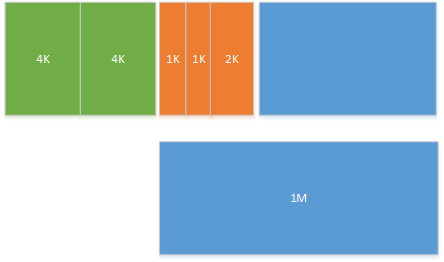
\includegraphics{../images/disk_layout.png}
    \caption{磁盘数据布局}
\end{figure}

磁盘头的元数据布局:MBR(0)+SB(1024)+DISKINFO(4096)。
其中SB包含定义的扩展属性:(cluster, node, type, disk, pool, cache, cached, cset)

每块盘的disk id属性,可用来重建disk/disk目录下的软链接。
block与info文件都可以通过读取磁盘头重建出来。bitmap文件则不可丢。

所在源文件是\emph{diskmd.c}。调用fnotify\_register监控磁盘目录的变化,进而添加或移除相应磁盘。

sqlite3划分为10个db文件,chkid信息hash到相应的db。每个db包含两个table:metadata和raw。

每个节点最多可以添加256个磁盘。

通过lich.node添加磁盘后,创建软链接,触发lichd的相关处理过程。

\begin{lstlisting}[frame=single]
CREATE TABLE metadata (key text primary key,
    disk integer,
    offset integer,
    parent text,
    priority integer,
    meta_version integer,
    fingerprint integer,
    wbdisk integer);

CREATE TABLE raw (key text primary key,
    disk integer,
    offset integer,
    parent text,
    priority integer,
    meta_version integer,
    fingerprint integer,
    wbdisk integer);
\end{lstlisting}

\subsection{状态机}

拔盘-恢复未完成,如何加入?(符号链接丢失,别的文件处在可用状态,重启lichd,修复符号链接)

拔盘-恢复完成,如何加入?

\subsection{Tier}

检测磁盘分层,支持两个磁盘分层:0和1, 0是SSD,1是HDD。

\section{Advanced}

NVMe

RDMA/DPDK/SPDK

AFA

\section{服务}

所有目录和卷的操作都经过相应的控制器,iscsi target与控制器之间存在映射关系。
命令行操作(不能部署在集群外的节点上)也是定位并连接到相应的控制器。

为了支持不同的应用层协议,扩展存储前端即可。存储引擎提供API。
\hl{以控制器为分界线,分为前端和后端}。

关于控制器,要解决定位、切换的问题。控制器发生切换后,上层应用收到\hl{EREMCHG错误},并重新寻址。
也要能主动地触发控制器的定向切换。

每个controller都bind到某一个cpu core上。每个core有独立的调度线程,
所谓bind到某个core上,就是插入该core调度器的相关队列里。

每个core分配有私有内存,尽量保持隔离性。

每个服务器节点的core数量必须相等,各节点上具有相同core hash的控制器构成corenet。
